\chapter{Computer Arithmetic: How Hardware Does Math}
\label{ch:arith}

A GPU is, more than anything, a machine for doing arithmetic: thousands of adders and multipliers working at once. NVIDIA's Ignite posting lists \emph{computer arithmetic} by name as a way to stand out. Chapter~\ref{ch:binary} showed how numbers are stored as bits, Chapter~\ref{ch:comb} built an adder, and Chapter~\ref{ch:gpu} introduced floating-point formats. This chapter puts those pieces to work: what happens when a result does not fit, how hardware shifts, adds quickly, multiplies and divides, how fractions are stored as fixed-point numbers, and how a floating-point unit actually adds and multiplies.

\begin{bigidea}
Every arithmetic circuit is a trade between three things: \textbf{speed} (how many gate delays from input to output), \textbf{area and power} (how many gates), and \textbf{accuracy} (how many bits, and how results are rounded). Faster adders and multipliers spend extra gates; smaller number formats save gates and energy by giving up precision.
\end{bigidea}

\section{When a result does not fit: carry, overflow and saturation}
\label{sec:overflow}

An $n$-bit adder always produces an $n$-bit result, plus a carry out of the top bit. The \emph{same} adder works for unsigned and for two's-complement signed numbers (Section~\ref{sec:twos}); only the meaning of ``the result did not fit'' differs.

\paragraph{Unsigned overflow: the carry.} For unsigned numbers, the result is too big exactly when there is a \term{carry out} of the most significant bit (MSB). In 8 bits, $200 + 100 = 300$, which does not fit in 0--255: the adder produces $300 - 256 = 44$ and a carry of 1.

\paragraph{Signed overflow: the overflow flag.} For signed numbers, the carry out means nothing on its own. Signed overflow happens when two numbers of the same sign produce a result of the opposite sign. Hardware detects it with one XOR gate:
\[
  V = c_{\text{into MSB}} \oplus c_{\text{out of MSB}}.
\]
If a carry goes into the sign bit but none comes out (or the reverse), the sign bit has been corrupted.

\begin{worked}{the four flags}
Add $0110\,0100$ (100) and $0011\,0010$ (50) in 8 bits. The result is $1001\,0110$.
\begin{itemize}
  \item As unsigned numbers: $100 + 50 = 150$, which fits in 0--255. There is no carry out, so $C = 0$, and $1001\,0110 = 150$ is correct.
  \item As signed numbers: $100 + 50 = 150$ does not fit in $-128$ to $127$. The result reads as $-106$. Bit 6 adds 1, 0 and an incoming carry, so a carry goes into the sign bit, but none comes out of it, so $V = 1$.
\end{itemize}
Processors record these as status \term{flags}: $C$ (carry), $V$ (overflow), $N$ (negative: the sign bit) and $Z$ (zero: every bit is 0). Here $C = 0$, $V = 1$, $N = 1$, $Z = 0$.
\end{worked}

\paragraph{Wrap or saturate?} When a result does not fit, ordinary integer hardware \term{wraps around}, keeping only the low $n$ bits. That is right for counters and addresses, but disastrous for a pixel brightness or an audio sample: a bright pixel that wraps becomes black. \term{Saturating arithmetic} instead clamps the result to the largest or smallest representable value.

\begin{center}
\begin{tabular}{lcc}
\toprule
8-bit operation & Wrapping result & Saturating result \\
\midrule
unsigned $200 + 100$ & 44 & 255 \\
unsigned $50 - 80$ & 226 & 0 \\
signed $100 + 50$ & $-106$ & 127 \\
signed $-100 - 50$ & 106 & $-128$ \\
\bottomrule
\end{tabular}
\end{center}

Saturation costs only a little logic: detect overflow ($C$ or $V$), and if it happened, select the maximum or minimum constant with a multiplexer instead of the adder's output. Digital signal processors, image pipelines and quantized neural-network hardware use it everywhere.

\begin{trap}
The carry flag is not the overflow flag. Adding $-1$ and $-1$ in 8 bits ($1111\,1111 + 1111\,1111$) produces a carry out, but the signed result $1111\,1110 = -2$ is perfectly correct, so $V = 0$.
\end{trap}

\section{Shifting}

\paragraph{Logical and arithmetic shifts.} Shifting left by $k$ multiplies by $2^k$ (if nothing falls off the top). Shifting right divides by $2^k$, and there are two kinds (Section~\ref{sec:bitops}): a \term{logical} right shift fills with zeros (for unsigned numbers), and an \term{arithmetic} right shift copies the sign bit in from the left, so negative numbers stay negative.

\begin{worked}{arithmetic shifts round down}
$-8$ in 8 bits is $1111\,1000$. Arithmetic right shift by 1: $1111\,1100 = -4$. Correct.

$-7$ is $1111\,1001$. Arithmetic right shift by 1: $1111\,1100 = -4$, not $-3$. An arithmetic shift rounds toward $-\infty$ (it computes $\lfloor -3.5 \rfloor = -4$), while integer division in C rounds toward zero ($-7/2 = -3$). Compilers add a small correction when they replace a signed division by a shift.
\end{worked}

\paragraph{The barrel shifter.} A processor must shift by any amount in a single cycle. A \term{barrel shifter} does it with $\log_2 n$ layers of 2:1 multiplexers. For a 32-bit value, the five bits of the shift amount control five layers that shift by 16, 8, 4, 2 and 1, each either shifting or passing the value straight through (Figure~\ref{fig:barrel}). Any amount from 0 to 31 is a sum of those powers of two. The cost: 5 layers of 32 multiplexers, 160 in all, but only five multiplexer delays.

\begin{figure}[h]
\centering
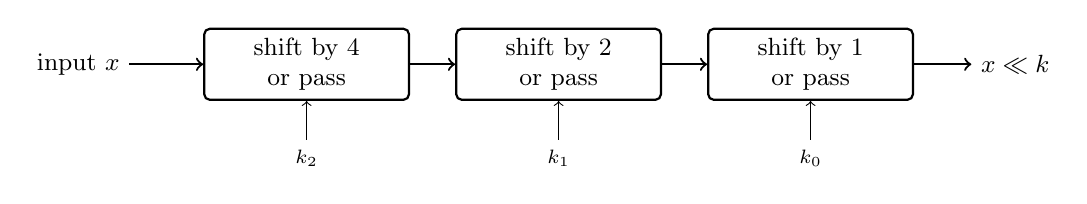
\begin{tikzpicture}[box/.style={draw,thick,rounded corners=2pt,minimum width=2.6cm,minimum height=0.8cm,font=\small,align=center}]
  \node[font=\small] (in) at (0,0) {input $x$};
  \node[box] (s4) at (2.9,0) {shift by 4\\or pass};
  \node[box] (s2) at (6.1,0) {shift by 2\\or pass};
  \node[box] (s1) at (9.3,0) {shift by 1\\or pass};
  \node[font=\small] (out) at (11.9,0) {$x \ll k$};
  \draw[->,thick] (in) -- (s4); \draw[->,thick] (s4) -- (s2); \draw[->,thick] (s2) -- (s1); \draw[->,thick] (s1) -- (out);
  \draw[<-] (s4.south) -- ++(0,-0.5) node[below,font=\scriptsize]{$k_2$};
  \draw[<-] (s2.south) -- ++(0,-0.5) node[below,font=\scriptsize]{$k_1$};
  \draw[<-] (s1.south) -- ++(0,-0.5) node[below,font=\scriptsize]{$k_0$};
\end{tikzpicture}
\caption{An 8-bit barrel shifter. Each layer is a row of 2:1 multiplexers controlled by one bit of the shift amount $k = k_2k_1k_0$. Shifting by 5 ($101_2$) means: shift by 4, pass, shift by 1.}
\label{fig:barrel}
\end{figure}

\paragraph{Multiplying by a constant.} Multiplying by a fixed number needs no multiplier at all, only shifts (which are free wiring) and adds:
\[
  10x = 8x + 2x = (x \ll 3) + (x \ll 1), \qquad 7x = 8x - x = (x \ll 3) - x.
\]
The second form uses a subtraction to replace two additions, the same trick Booth recoding uses below.

\section{Adding faster}
\label{sec:fastadd}

Chapter~\ref{ch:comb} built a ripple-carry adder: simple, but the carry may have to travel through every bit, so a 64-bit add takes 64 full-adder delays. Faster adders break that chain.

\paragraph{Generate and propagate.} For bit $i$, define
\begin{align*}
  G_i &= A_i B_i && \text{(this bit generates a carry: both bits are 1)}, \\
  P_i &= A_i \oplus B_i && \text{(this bit propagates an incoming carry: exactly one bit is 1)}.
\end{align*}
Then the carry out of bit $i$ is $c_{i+1} = G_i + P_i c_i$: a carry leaves bit $i$ if the bit makes one, or passes one along. Substituting each equation into the next gives every carry directly from the inputs:
\begin{align*}
  c_1 &= G_0 + P_0 c_0 \\
  c_2 &= G_1 + P_1 G_0 + P_1 P_0 c_0 \\
  c_3 &= G_2 + P_2 G_1 + P_2 P_1 G_0 + P_2 P_1 P_0 c_0 \\
  c_4 &= G_3 + P_3 G_2 + P_3 P_2 G_1 + P_3 P_2 P_1 G_0 + P_3 P_2 P_1 P_0 c_0
\end{align*}
Each line is just AND gates feeding an OR gate, so all four carries are ready after about two gate delays instead of four full-adder delays. This is a 4-bit \term{carry-lookahead adder} (CLA). The equations grow quickly, so wide adders apply the same idea in a tree: each 4-bit group computes a group generate and group propagate, and a second level of lookahead combines groups. \term{Prefix adders} (Kogge--Stone, Brent--Kung) are the systematic version, with delay growing as $\log_2 n$: about 6 levels for 64 bits instead of 64 stages.

\paragraph{Carry-select.} Compute the upper half of the sum twice, once assuming its carry-in is 0 and once assuming 1, while the lower half is still adding. When the real carry arrives, a multiplexer picks the right upper half. Speed for area: roughly double the adder hardware for the upper half.

\paragraph{Carry-save: adding three numbers without carrying.} A row of independent full adders takes three numbers and produces \emph{two}: a sum vector (each bit's $A \oplus B \oplus C$) and a carry vector (each bit's majority, shifted left one place). No carry travels sideways, so the delay is one full adder no matter how wide the numbers are. This \term{carry-save adder} (CSA), also called a 3:2 compressor, is the key to fast multipliers.

\begin{worked}{carry-save addition}
Add 5, 6 and 7 ($101$, $110$, $111$).
Sum vector: bitwise XOR of all three $= 100 = 4$.
Carry vector: bitwise majority $= 111$, shifted left $= 1110 = 14$.
One ordinary addition finishes the job: $4 + 14 = 18 = 5 + 6 + 7$. Reducing three numbers to two cost one full-adder delay; only the final addition needs a carry chain.
\end{worked}

\section{Multiplication}
\label{sec:mult}

\paragraph{Shift and add.} Binary multiplication is the long multiplication taught in school, but easier, because each digit of the multiplier is 0 or 1: each \term{partial product} is either zero or a shifted copy of the multiplicand.

\begin{worked}{$11 \times 13$ in binary}
\begin{center}
\begin{tabular}{rl}
\code{\ \ \ \ 1011} & multiplicand $= 11$ \\
$\times$\ \code{\ \ \ \ 1101} & multiplier $= 13$ \\
\midrule
\code{\ \ \ \ 1011} & bit 0 is 1: $11$ \\
\code{\ \ \ 0000\ } & bit 1 is 0: $0$ \\
\code{\ \ 1011\ \ } & bit 2 is 1: $11 \times 4 = 44$ \\
\code{\ 1011\ \ \ } & bit 3 is 1: $11 \times 8 = 88$ \\
\midrule
\code{10001111} & $11 + 44 + 88 = 143$ \\
\end{tabular}
\end{center}
Each partial-product bit is one AND gate (multiplicand bit AND multiplier bit). Multiplying an $n$-bit number by an $m$-bit number gives up to $n + m$ bits: here $4 + 4 = 8$, and indeed $15 \times 15 = 225$ needs all 8.
\end{worked}

\paragraph{Array multipliers and trees.} An $n \times n$ multiplier makes $n$ partial products from $n^2$ AND gates, then adds them up. An \term{array multiplier} adds them row by row in a grid of full adders: regular and easy to lay out, with delay that grows in proportion to $n$. A \term{Wallace tree} or \term{Dadda tree} instead feeds the partial products through layers of carry-save adders, each layer turning every three rows into two. The row count falls by about a third per layer, so $n$ rows shrink to two in about $\log_{1.5} n$ layers, and one fast adder from Section~\ref{sec:fastadd} produces the product. For 24 rows (an FP32 significand) that is 7 layers.

\paragraph{Booth recoding: fewer partial products.} Long runs of 1s are wasteful: $0111_2 = 7$ needs three partial products, but $7 = 8 - 1$ needs only two (a shifted copy and a subtracted copy). \term{Radix-4 Booth recoding} applies this systematically. It looks at the multiplier in overlapping groups of three bits $(b_{2i+1}, b_{2i}, b_{2i-1})$, with $b_{-1} = 0$, and turns each group into one digit:
\[
  d_i = -2\,b_{2i+1} + b_{2i} + b_{2i-1} \in \{-2, -1, 0, +1, +2\}.
\]
The multiplier then equals $\sum_i d_i \, 4^i$, so an $n$-bit multiplier needs only about $n/2$ partial products. Each is $0$, $\pm M$ or $\pm 2M$ (a shift), and negation is invert-plus-one, so they are cheap to make. Booth recoding also handles two's-complement (signed) multipliers with no special cases.

\begin{center}
\begin{tabular}{ccc|c|l}
\toprule
$b_{2i+1}$ & $b_{2i}$ & $b_{2i-1}$ & digit $d_i$ & partial product \\
\midrule
0 & 0 & 0 & $0$ & 0 \\
0 & 0 & 1 & $+1$ & $+M$ \\
0 & 1 & 0 & $+1$ & $+M$ \\
0 & 1 & 1 & $+2$ & $+2M$ (shift left) \\
1 & 0 & 0 & $-2$ & $-2M$ \\
1 & 0 & 1 & $-1$ & $-M$ \\
1 & 1 & 0 & $-1$ & $-M$ \\
1 & 1 & 1 & $0$ & 0 \\
\bottomrule
\end{tabular}
\end{center}

\begin{worked}{Booth-recoding 7}
The multiplier is $0111$, so $b_3 b_2 b_1 b_0 = 0111$ and $b_{-1} = 0$.
Group 0 is $(b_1, b_0, b_{-1}) = (1, 1, 0)$: $d_0 = -2 + 1 + 0 = -1$.
Group 1 is $(b_3, b_2, b_1) = (0, 1, 1)$: $d_1 = 0 + 1 + 1 = +2$.
Check: $d_1 \cdot 4 + d_0 = 8 - 1 = 7$. So $7M = 2M \cdot 4 - M$: two partial products instead of three.
\end{worked}

\paragraph{Why multipliers dominate AI hardware.} An $n \times n$ multiplier needs about $n^2$ partial-product bits, so its area and energy grow roughly with the \emph{square} of the width. An FP32 multiplier multiplies 24-bit significands; BF16 multiplies 8-bit ones (Chapter~\ref{ch:gpu}), so its multiplier is roughly $(24/8)^2 = 9$ times smaller. That, together with moving fewer bytes, is why tensor cores use narrow formats. A \term{multiply-accumulate} (MAC) unit, which computes $acc \leftarrow acc + a \times b$, is the building block of every tensor core and systolic array.

\section{Division}

Division is the slow operation. Binary long division produces \emph{one quotient bit per step}, and each step depends on the remainder from the previous one, so it cannot be done in parallel like a multiplier's partial products.

\paragraph{Restoring division.} Start with a remainder of 0. For each dividend bit, from the most significant down: shift the remainder left and bring in the next bit; if the remainder is now at least the divisor, subtract the divisor and write a quotient bit of 1, otherwise write 0. (The name comes from hardware that subtracts first and adds the divisor back, ``restoring,'' if the result went negative.)

\begin{worked}{$13 \div 3$}
Dividend $1101$, divisor $3$.
\begin{center}
\begin{tabular}{cccc}
\toprule
Bit brought in & Remainder & $\ge 3$? & Quotient bit \\
\midrule
1 & 1 & no & 0 \\
1 & $2 \cdot 1 + 1 = 3$ & yes, $3 - 3 = 0$ & 1 \\
0 & $2 \cdot 0 + 0 = 0$ & no & 0 \\
1 & $2 \cdot 0 + 1 = 1$ & no & 0 \\
\bottomrule
\end{tabular}
\end{center}
Quotient $0100 = 4$, remainder 1. Indeed $13 = 4 \times 3 + 1$.
\end{worked}

A 32-bit divide takes on the order of 32 steps. Faster dividers (SRT division) produce two or more quotient bits per step, and GPUs usually compute a reciprocal approximation from a small table and refine it with a couple of multiply-add iterations (Newton--Raphson), because multipliers are plentiful and fast.

\paragraph{Dividing by a constant.} Compilers and hardware avoid division by a known constant entirely: they multiply by a scaled reciprocal and shift. For any 16-bit unsigned $x$, $x / 3 = (x \times 43691) \gg 17$, because $43691 \approx 2^{17}/3$. A multiply and a shift replace a 16-step division.

\section{Fixed point: fractions on integer hardware}
\label{sec:fixed}

Integer hardware is small and fast, and many signals, such as audio samples, filter coefficients and neural-network weights, have a known, limited range. \term{Fixed-point} numbers store fractions in ordinary integers by agreeing on where the binary point is.

\begin{defn}{Q format}
A \textbf{Q$m$.$n$} number has $m$ integer bits and $n$ fraction bits. Its value is the stored integer divided by $2^n$. The \textbf{resolution} (the step between neighbouring values) is $2^{-n}$. For signed numbers, the sign is counted in $m$, so signed Q1.7 is 8 bits covering $-1$ to $1 - 2^{-7}$.
\end{defn}

\begin{worked}{reading and writing Q formats}
Unsigned Q4.4 pattern $0010\,1100$: integer part $0010 = 2$, fraction part $1100 = 12/16 = 0.75$, value 2.75. (Equivalently, $44 / 2^4 = 2.75$.)

Store 0.3 in signed Q1.7: $0.3 \times 2^7 = 38.4$, which rounds to 38. The stored value is $38/128 = 0.296875$, an error of about 0.003. The worst-case rounding error is half a step, $2^{-8} \approx 0.0039$.
\end{worked}

\paragraph{Arithmetic in fixed point.}
\begin{itemize}
  \item \textbf{Adding} needs both numbers in the same format, with their binary points lined up: shift one of them first if needed. Then it is a plain integer add (watch for overflow, and consider saturation).
  \item \textbf{Multiplying} two integers multiplies the scale factors too: a Q$a$.$b$ number times a Q$c$.$d$ number gives a Q$(a{+}c)$.$(b{+}d)$ product. To return to $b$ fraction bits, shift right by $d$, ideally rounding rather than truncating.
\end{itemize}

\begin{worked}{multiplying in Q1.7}
$0.5$ is stored as $64$ and $0.25$ as $32$ (both Q1.7). The integer product is $64 \times 32 = 2048$, a Q2.14 number. Shift right by 7: $2048 / 128 = 16$, which is $16/128 = 0.125$ in Q1.7. Correct: $0.5 \times 0.25 = 0.125$.
\end{worked}

\paragraph{Quantization for AI.} Neural-network inference often stores weights and activations as INT8 with a \term{scale factor} (and sometimes a zero point): $\text{real value} \approx s \times (q - z)$, where $q$ is the stored 8-bit integer. The scale is chosen per tensor or per channel so that the 256 available levels cover the values that actually occur. The multiply-adds run on cheap integer hardware with wide (32-bit) accumulators, and the result is rescaled at the end.

\section{Floating-point arithmetic}
\label{sec:fparith}

Chapter~\ref{ch:gpu} showed how a floating-point number is stored: sign $s$, exponent $e$ and fraction $m$, with value $(-1)^s \times 1.m \times 2^{e - 127}$ in FP32. Fixed point has a constant step size; floating point keeps a constant number of \emph{significant bits}, so it covers huge and tiny numbers alike. The cost is that every operation must line up exponents, renormalize and round.

\paragraph{Special values.} The smallest and largest exponent fields are reserved:
\begin{center}
\begin{tabular}{lll}
\toprule
Exponent field (FP32) & Fraction & Meaning \\
\midrule
1 to 254 & anything & normal number $1.m \times 2^{e-127}$ \\
0 & 0 & zero ($+0$ or $-0$) \\
0 & not 0 & subnormal number $0.m \times 2^{-126}$ \\
255 & 0 & $+\infty$ or $-\infty$ \\
255 & not 0 & NaN (not a number) \\
\bottomrule
\end{tabular}
\end{center}
Overflow gives $\pm\infty$; $1/0$ gives $+\infty$; $0/0$ and $\infty - \infty$ give NaN. NaN spreads through every later operation, and it is not equal to anything, not even itself.

\paragraph{Subnormal numbers.} The smallest normal FP32 number is $2^{-126} \approx 1.2\times10^{-38}$. Without subnormals, the next value down would be zero, and $x - y$ could be 0 even when $x \ne y$. \term{Subnormal} (denormal) numbers drop the hidden leading 1 to fill that gap evenly, down to $2^{-149} \approx 1.4\times10^{-45}$. This \term{gradual underflow} keeps small differences from vanishing. Handling subnormals takes extra hardware or time, so some processors offer \term{flush-to-zero} modes that replace them with 0 for speed; CUDA has such an option.

\paragraph{Precision.} With 23 stored fraction bits plus the hidden 1, FP32 has 24 significant bits. The gap between 1.0 and the next larger FP32 number is $2^{-23} \approx 1.2\times10^{-7}$ (\term{machine epsilon}), about 7 decimal digits of precision. The gap between neighbouring numbers is called a \term{ULP} (unit in the last place), and it grows with the number's size: between $2^{26}$ and $2^{27}$ the FP32 spacing is $2^{26-23} = 8$.

\subsection*{Floating-point addition}

\begin{figure}[h]
\centering
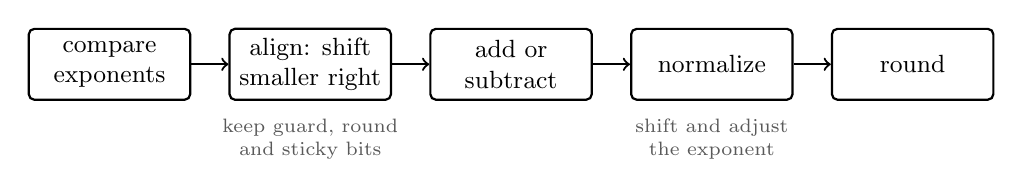
\begin{tikzpicture}[box/.style={draw,thick,rounded corners=2pt,minimum width=2.05cm,minimum height=0.9cm,font=\small,align=center}]
  \node[box] (a) at (0,0) {compare\\exponents};
  \node[box] (b) at (2.55,0) {align: shift\\smaller right};
  \node[box] (c) at (5.1,0) {add or\\subtract};
  \node[box] (d) at (7.65,0) {normalize};
  \node[box] (e) at (10.2,0) {round};
  \draw[->,thick] (a) -- (b); \draw[->,thick] (b) -- (c); \draw[->,thick] (c) -- (d); \draw[->,thick] (d) -- (e);
  \node[font=\scriptsize,gray!70!black,align=center] at (2.55,-0.95) {keep guard, round\\and sticky bits};
  \node[font=\scriptsize,gray!70!black,align=center] at (7.65,-0.95) {shift and adjust\\the exponent};
\end{tikzpicture}
\caption{The steps of a floating-point adder. Hardware pipelines these steps over several clock cycles.}
\label{fig:fpadd}
\end{figure}

\begin{enumerate}
  \item \textbf{Compare exponents.} The number with the smaller exponent must be adjusted to match the larger.
  \item \textbf{Align.} Shift the smaller number's significand right by the exponent difference.
  \item \textbf{Add or subtract} the significands (subtract if the signs differ).
  \item \textbf{Normalize.} Shift the result so it again has the form $1.xxx$, adjusting the exponent: one place right if the sum reached 2 or more, possibly many places left if a subtraction cancelled the leading bits.
  \item \textbf{Round} back to 23 fraction bits, and check for overflow, underflow and special values.
\end{enumerate}

\begin{worked}{$3.0 + 0.5$}
$3.0 = 1.1_2 \times 2^1$ and $0.5 = 1.0_2 \times 2^{-1}$. The exponents differ by 2, so shift the smaller significand right by 2: $1.0_2 \times 2^{-1} = 0.01_2 \times 2^1$. Add: $1.10_2 + 0.01_2 = 1.11_2$, so the result is $1.11_2 \times 2^1 = 3.5$. Already normalized; nothing to round.
\end{worked}

\paragraph{Guard, round and sticky bits.} During alignment, bits shifted off the right end are not simply thrown away. The adder keeps the first two of them (the \term{guard} and \term{round} bits) and ORs all the rest into one \term{sticky} bit (``was anything nonzero shifted out?''). Those three extra bits are exactly enough to round correctly, as if the exact result had been computed with infinite precision.

\subsection*{Floating-point multiplication}

Multiplication is simpler than addition because no alignment is needed:
\begin{enumerate}
  \item \textbf{Sign:} XOR of the two signs.
  \item \textbf{Exponent:} add the exponent fields and subtract one bias: $e = e_1 + e_2 - 127$.
  \item \textbf{Significand:} multiply the two 24-bit significands (a $24 \times 24$ integer multiplier, Section~\ref{sec:mult}). The product lies between 1 and 4.
  \item \textbf{Normalize} (shift right once if the product is 2 or more, and add 1 to the exponent), then \textbf{round}.
\end{enumerate}

\begin{worked}{$3.0 \times 2.5$}
$3.0 = 1.1_2 \times 2^1$ (exponent field 128) and $2.5 = 1.01_2 \times 2^1$ (exponent field 128). Sign: $0 \oplus 0 = 0$. Exponent field: $128 + 128 - 127 = 129$, meaning $2^2$. Significands: $1.1_2 \times 1.01_2 = 1.111_2$ (that is, $1.5 \times 1.25 = 1.875$). Result: $1.111_2 \times 2^2 = 7.5$. Correct.
\end{worked}

\subsection*{Rounding}

The exact result of an operation usually falls between two representable numbers, and the \term{rounding mode} picks one. IEEE 754 defines four:
\begin{itemize}
  \item \textbf{Round to nearest, ties to even} (the default): pick the nearer neighbour; on an exact tie, pick the one whose last bit is 0. In decimal terms, 2.5 rounds to 2 and 3.5 to 4. Always rounding ties upward would bias long sums upward; ties to even makes the errors cancel on average.
  \item \textbf{Toward zero} (truncation), \textbf{toward $+\infty$}, and \textbf{toward $-\infty$}: used for special purposes such as interval arithmetic.
\end{itemize}

\paragraph{Floating-point addition is not associative.} Because every operation rounds, the order of operations changes the result.

\begin{worked}{order matters}
In FP32, numbers near $10^8$ are spaced 8 apart ($10^8$ lies between $2^{26}$ and $2^{27}$). So $10^8 + 1$ rounds back to $10^8$, and
\[
  (10^8 + 1) - 10^8 = 0, \qquad\text{but}\qquad (10^8 - 10^8) + 1 = 1.
\]
A GPU that sums a million numbers in parallel adds them in a different order than a CPU loop does, so the two answers can differ in the last bits. Neither is ``wrong.'' This matters when verifying GPU arithmetic: results are compared within a tolerance, not bit for bit, unless the order is fixed.
\end{worked}

\paragraph{Fused multiply-add.} A \term{fused multiply-add} (FMA) computes $a \times b + c$ with a \emph{single} rounding at the end, instead of rounding the product and then the sum. It is both faster (one instruction) and more accurate. Modern GPUs and CPUs build their floating-point units around FMA, and a tensor core is essentially a block of multiply-adds.

\paragraph{Mixed precision.} AI hardware multiplies in a narrow format (FP16, BF16, FP8) but \emph{accumulates} in FP32. A long sum of small products in a narrow format would lose the small terms, exactly as in the $10^8 + 1$ example; a wide accumulator keeps them.

\section{How arithmetic hardware is checked}

An arithmetic unit has far too many inputs to test exhaustively (a 32-bit adder has $2^{64}$ input pairs). It is verified by comparing it against a \term{reference model}, a simple program that computes the right answer (Section~\ref{sec:verif}), using millions of random inputs plus the \term{corner cases} where bugs hide: zero, one, the largest and smallest values, values that overflow, and, for floating point, $\pm 0$, $\pm\infty$, NaN, subnormals and results that fall exactly halfway between two representable numbers. Formal tools can prove an adder correct for all inputs; multipliers are hard even for formal tools and need special techniques.

\section{Summary}

\begin{itemize}
  \item Unsigned overflow is the carry out of the MSB; signed overflow is $V = c_{\text{into MSB}} \oplus c_{\text{out of MSB}}$. Saturating arithmetic clamps instead of wrapping.
  \item An arithmetic right shift rounds toward $-\infty$. A barrel shifter shifts any amount with $\log_2 n$ layers of multiplexers. Constant multiplies are shifts and adds.
  \item Carry-lookahead and prefix adders compute carries from $G_i = A_iB_i$ and $P_i = A_i \oplus B_i$ in $O(\log n)$ delay. A carry-save adder turns three numbers into two with one full-adder delay.
  \item An $n \times m$ multiply gives $n + m$ bits. Partial products are summed with arrays or Wallace/Dadda trees; radix-4 Booth recoding halves their number. Multiplier area grows roughly with width squared.
  \item Division produces one quotient bit per step (restoring division); division by a constant becomes a multiply and shift.
  \item Q$m$.$n$ fixed point: value $=$ integer $/2^n$, resolution $2^{-n}$; Q$a$.$b \times$ Q$c$.$d$ gives $b + d$ fraction bits. INT8 quantization uses a scale factor.
  \item Floating-point add: compare exponents, align, add, normalize, round (with guard, round and sticky bits). Multiply: XOR signs, add exponents minus the bias, multiply significands, normalize, round.
  \item Special values: $\pm 0$, $\pm\infty$, NaN, and subnormals (gradual underflow). FP32 epsilon is $2^{-23}$. Default rounding is round to nearest, ties to even. FP addition is not associative. FMA rounds once.
\end{itemize}

\section{Exercises}

\begin{enumerate}
  \item Add $0111\,0000$ and $0101\,0000$ in 8 bits. What is the 8-bit result, and what are the carry ($C$) and overflow ($V$) flags?
  \item What does 8-bit unsigned saturating arithmetic give for $250 + 10$? And for $5 - 9$?
  \item What is $-9$ (8 bits) arithmetically shifted right by 1? How does that differ from $-9/2$ in C?
  \item How many layers of 2:1 multiplexers does a 64-bit barrel shifter need?
  \item Write $c_2$ for a carry-lookahead adder in terms of $G_0$, $G_1$, $P_0$, $P_1$ and $c_0$.
  \item A carry-save adder adds 9, 5 and 3. What are the sum vector and the carry vector? Check that they add to 17.
  \item How many bits does the product of a 12-bit and an 8-bit unsigned number need?
  \item Booth-recode the 4-bit multiplier $0110$ (6) into radix-4 digits.
  \item Divide $1110$ (14) by 4 with restoring division. What are the quotient and remainder?
  \item What value does unsigned Q4.4 $0101\,1010$ represent? What is the resolution of Q4.4?
  \item A Q2.6 number is multiplied by a Q3.5 number. How many integer and fraction bits does the full product have?
  \item Add $1.5$ and $0.375$ in floating point, step by step.
  \item In FP32, multiply $1.5 \times 2^{3}$ by $1.5 \times 2^{-1}$. What are the result's exponent field and value?
  \item Name the five kinds of value an FP32 exponent field can indicate. What is $0/0$?
  \item Why does IEEE 754 round ties to even instead of always rounding ties up?
  \item Give one reason a tensor core uses BF16 or FP8 multipliers but accumulates in FP32.
\end{enumerate}

\subsection*{Answers}
\begin{enumerate}
  \item $112 + 80 = 192$: the result is $1100\,0000$. No carry out of the MSB, so $C = 0$ (as unsigned, 192 is correct). A carry went into the sign bit but none came out, so $V = 1$ (as signed, the result $-64$ is wrong).
  \item 255 (instead of wrapping to 4), and 0 (instead of wrapping to 252).
  \item $-9 = 1111\,0111$; shifted: $1111\,1011 = -5$ (rounds toward $-\infty$). C's $-9/2$ gives $-4$ (rounds toward zero).
  \item $\log_2 64 = 6$ layers (shifts of 32, 16, 8, 4, 2 and 1).
  \item $c_2 = G_1 + P_1 G_0 + P_1 P_0 c_0$.
  \item $9 = 1001$, $5 = 0101$, $3 = 0011$. Sum vector (XOR) $= 1111 = 15$. Majority $= 0001$, shifted left $= 0010 = 2$. $15 + 2 = 17$.
  \item $12 + 8 = 20$ bits.
  \item $b_3 b_2 b_1 b_0 = 0110$, $b_{-1} = 0$. Group 0, $(b_1, b_0, b_{-1}) = (1, 0, 0)$: $d_0 = -2$. Group 1, $(b_3, b_2, b_1) = (0, 1, 1)$: $d_1 = +2$. Check: $2 \times 4 - 2 = 6$.
  \item Quotient 3 ($0011$), remainder 2. Step by step: remainders 1, 3, 7 ($\ge 4$, so subtract: 3, quotient bit 1), then 6 ($\ge 4$, subtract: 2, quotient bit 1); quotient bits $0011$.
  \item $0101 = 5$ and $1010/16 = 0.625$, so 5.625. Resolution $2^{-4} = 0.0625$.
  \item $2 + 3 = 5$ integer bits and $6 + 5 = 11$ fraction bits (16 bits in all).
  \item $1.5 = 1.1_2 \times 2^0$ and $0.375 = 1.1_2 \times 2^{-2}$. Align: $1.1_2 \times 2^{-2} = 0.011_2 \times 2^0$. Add: $1.100_2 + 0.011_2 = 1.111_2$, so $1.111_2 \times 2^0 = 1.875$.
  \item Exponent: $3 + (-1) = 2$, field $130 + 126 - 127 = 129$. Significands: $1.5 \times 1.5 = 2.25$, which is $\ge 2$, so normalize to $1.125 \times 2^1$ and add 1 to the exponent: field 130, value $1.125 \times 2^3 = 9$. Check: $12 \times 0.75 = 9$.
  \item Normal numbers, zero, subnormal numbers, infinity and NaN. $0/0$ is NaN.
  \item Always rounding ties up biases results upward, and in long computations the bias accumulates. Ties to even rounds up half the time and down half the time, so the errors cancel on average.
  \item Narrow multipliers are far smaller and cheaper (area grows roughly with the significand width squared) and move fewer bytes; but a long sum in a narrow format would lose small terms to rounding, so the accumulator stays FP32.
\end{enumerate}
